Beispielausgaben aller auf bwinf.de zur Verfügung gestellten Beispiele finden sie im .zip.

Hier finden Sie die Ausgaben, auf denen ein Rhinozelfant gefunden wurde. Die Bilder auf denen kein Rhinozelfant gefunden wurde, entsprechen zu 100\% den Eingabebildern.

\subsection{Beispiel 1}
	\centering
	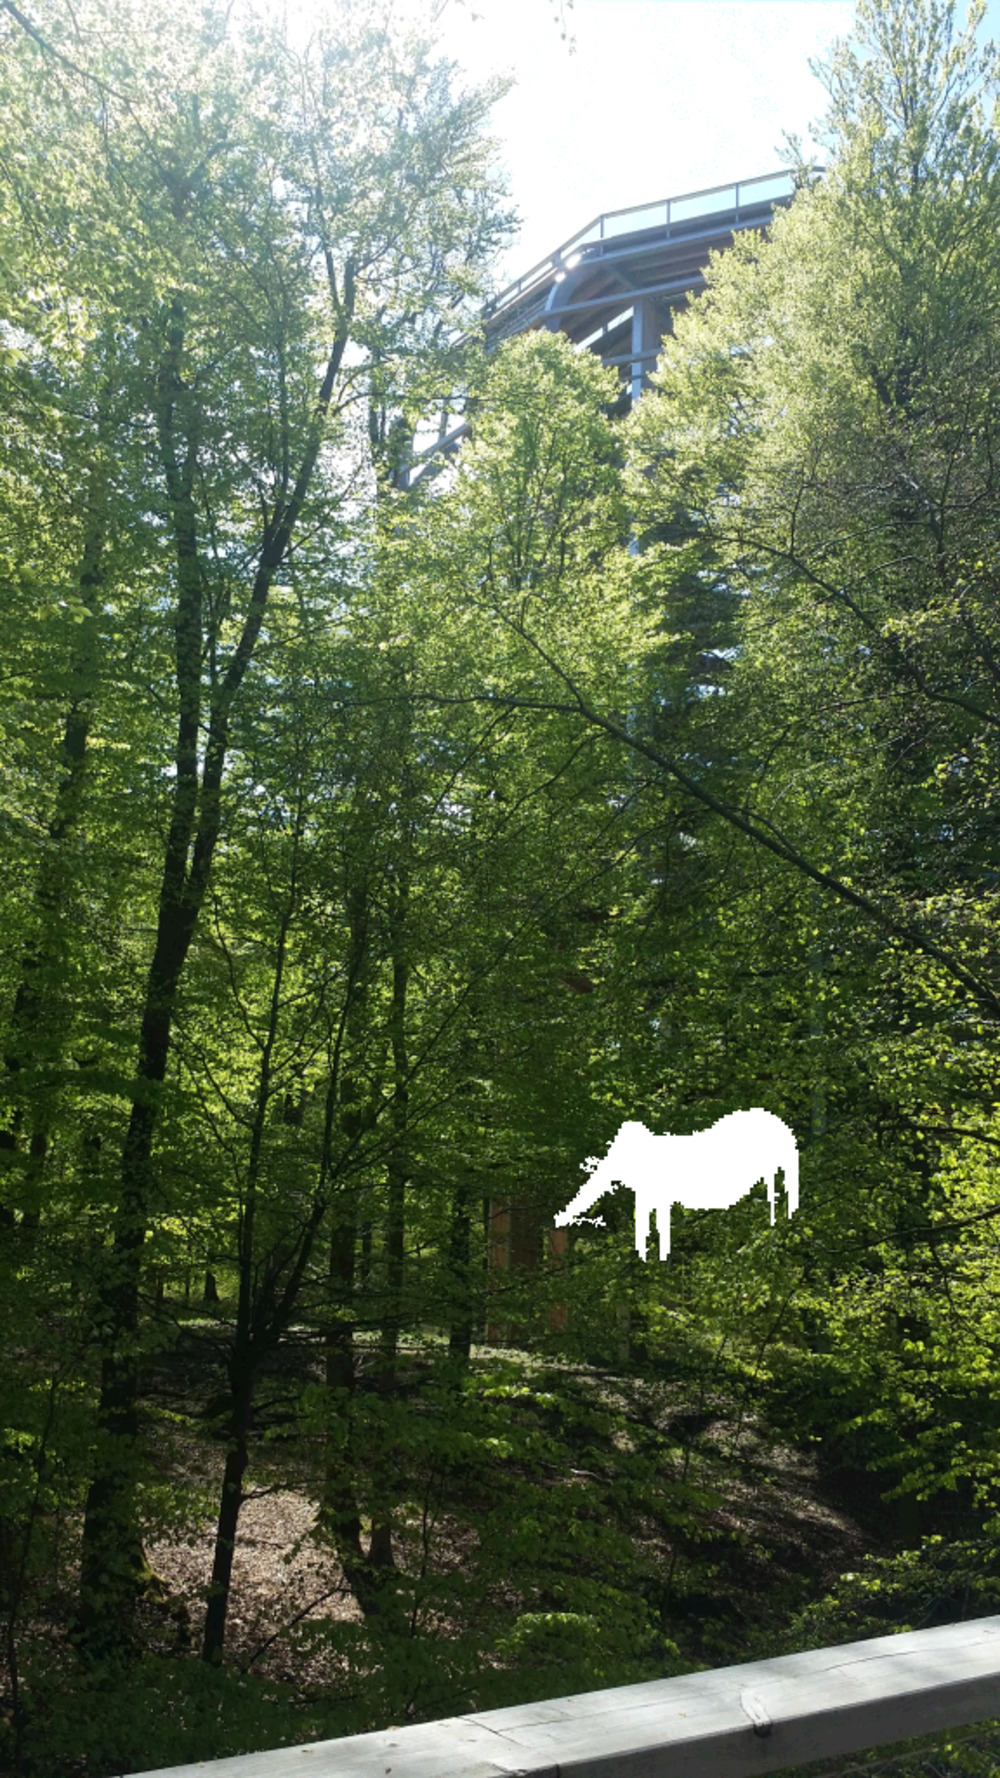
\includegraphics[width=0.45\textwidth]{bsp-0}
\subsection{Beispiel 2}
	\centering
	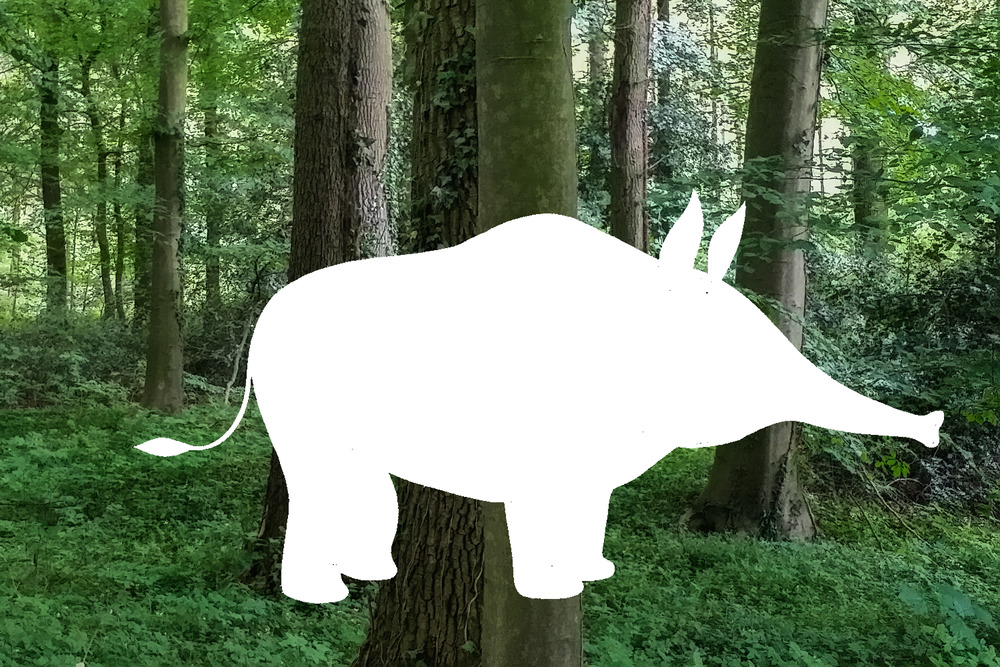
\includegraphics[width=0.45\textwidth]{bsp-1}
\subsection{Beispiel 4}
	\centering
	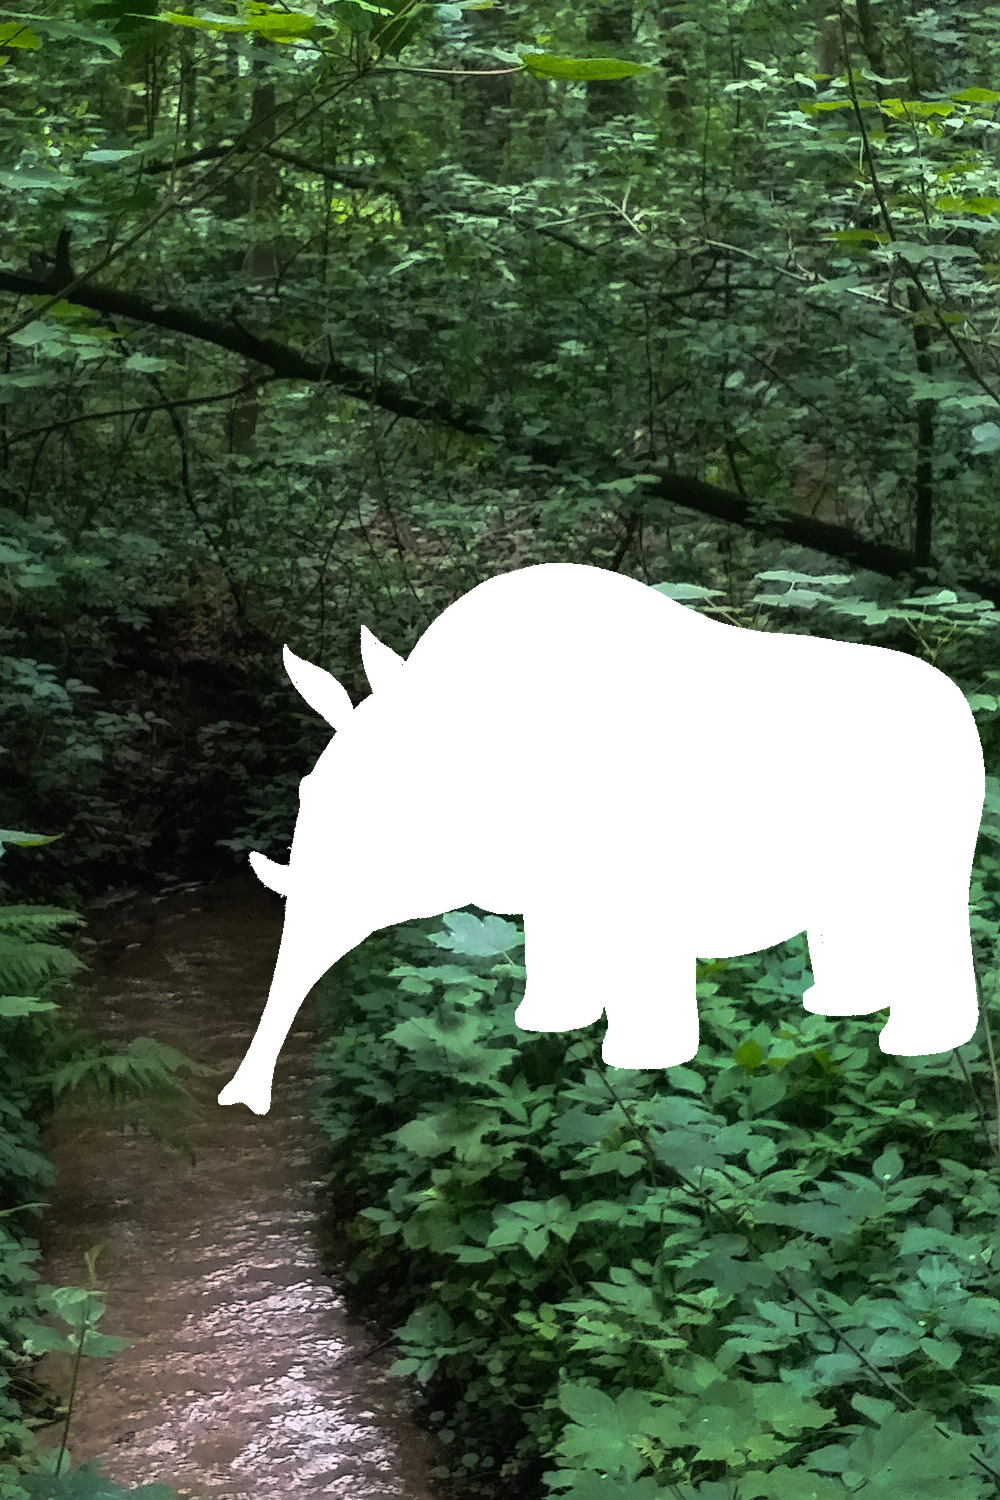
\includegraphics[width=0.45\textwidth]{bsp-2}
\subsection{Beispiel 8}
	\centering
	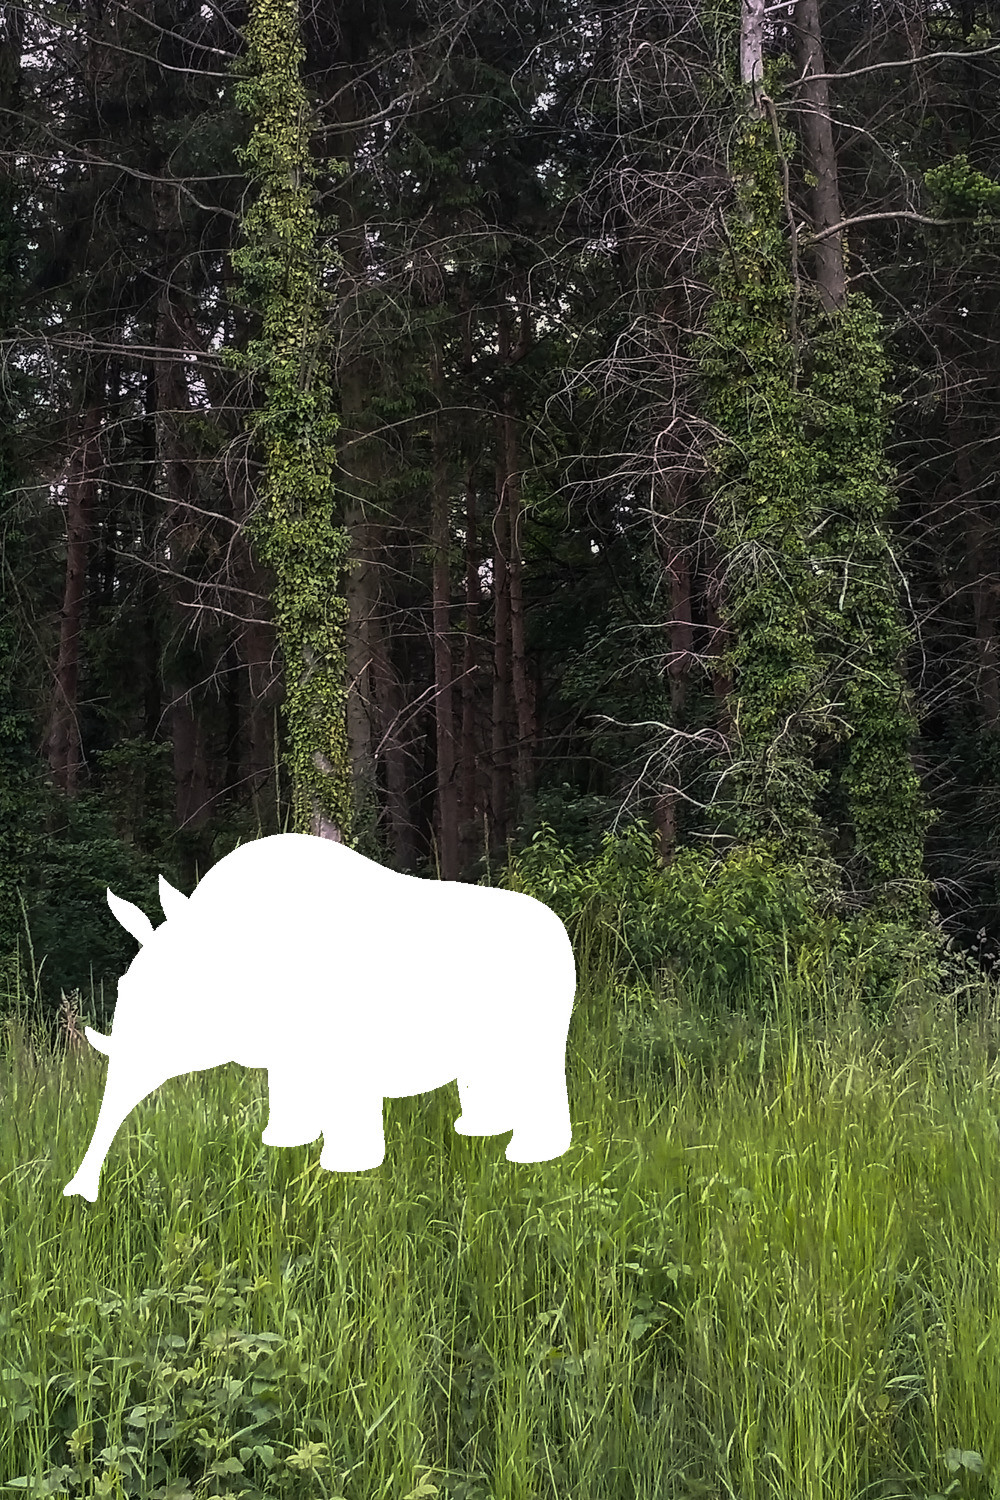
\includegraphics[width=0.45\textwidth]{bsp-3}
\subsection{Beispiel 9}
	\centering
	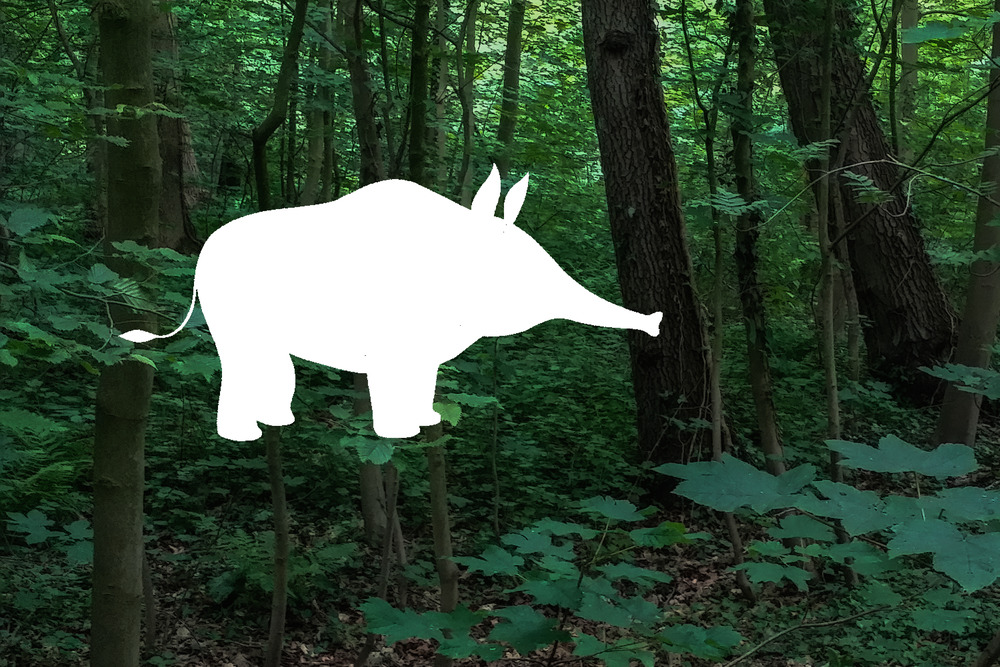
\includegraphics[width=0.45\textwidth]{bsp-4}

% Hier einige Beispiel mit Kommentar:

% \subsection{Beispiel 1}

% \begin{figure}[h]
% 	\centering
% 	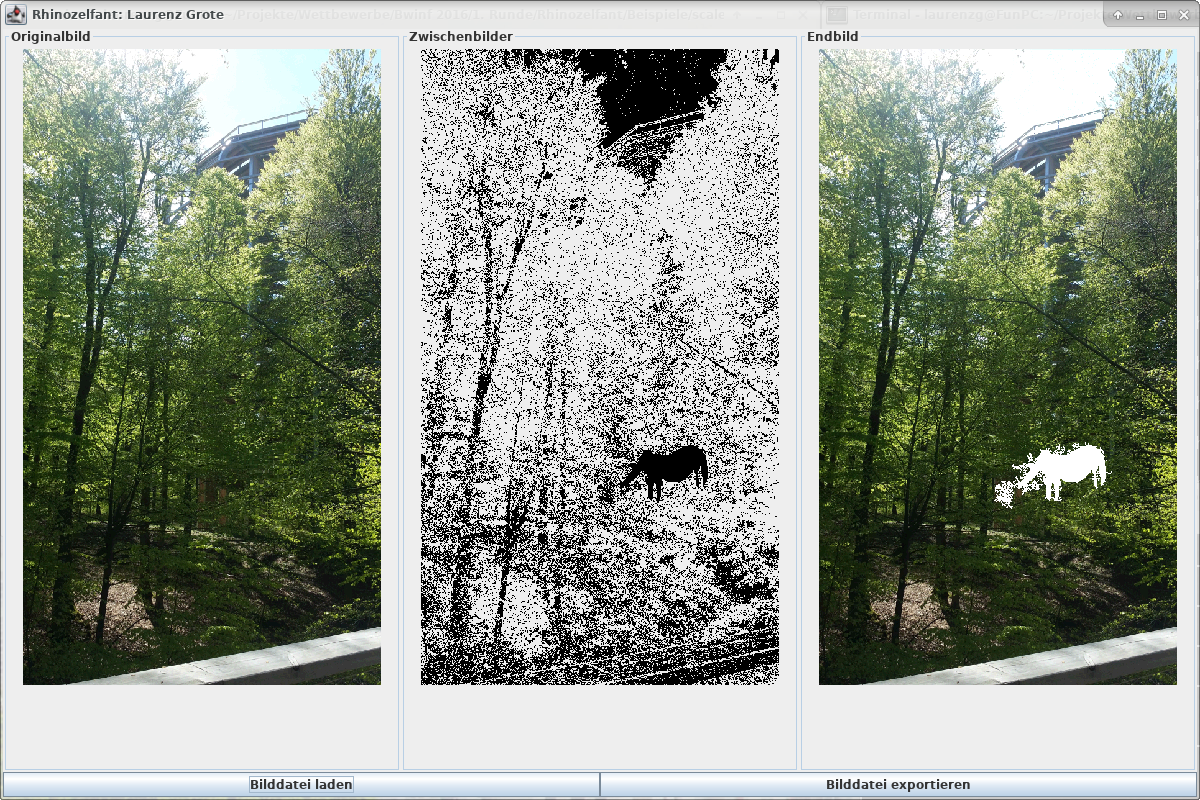
\includegraphics[width=0.8\textwidth]{bsp1}
% 	\caption {Beispielbild 1}
% \end{figure}

% In diesem Bild gibt es neben dem schon erkennbaren Rhinozelfanten einige monotone Bereiche an der Brücke, im Himmel und an den Baumstämmen (siehe Zwischenbild).

% Die meisten der Baumstämme werden wegen nicht ausreichender Breite schon im ersten Filter ausgefiltert, das Brückengeländer erfüllt die Mindesthöhe wegen der zahlreichen weißen, das Rechteck unterbrechenden Felder nicht. Im Himmel gibt es einige Stellen die die ersten beiden Felder durchlaufen, jedoch liegen keine Beine vorher. Daher zeichnet das Programm nur den einen Rhinozelfanten im Endbild ein.

% Leider wird an den Rüssel noch einige Stellen eingezeichnet, die nicht zum Elefanten gehören. Dies liegt daran dass einige Waldstellen direkt an den Elefanten anschließen. Da dies nur bei einem Beispiel in diesem Maße auftrat, habe ich mich dagegen entschieden, einen weiteren Algorithmus zur Entfernung des Umgebungsrauschens zu programmieren.

% \subsection{Beispiel 3}

% \begin{figure}[h]
% 	\centering
% 	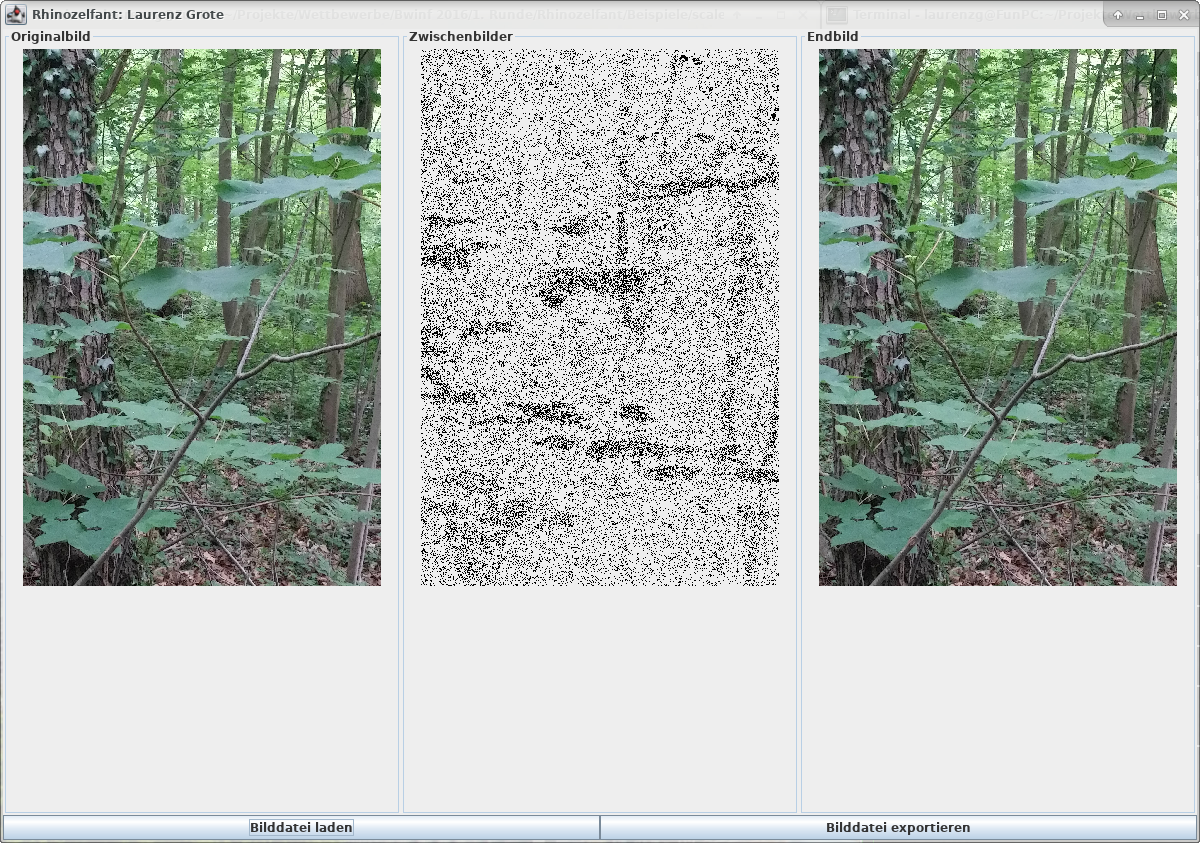
\includegraphics[width=0.8\textwidth]{bsp3}
% 	\caption {Beispielbild 3}
% \end{figure}

% In diesem Bild liegen nur durch die Blätter im Vordergrund einige gleichfarbige Stellen vor, korrekterweise zeichnet das Programm jedoch keine Rhinozelfanten ein.

% \subsection{Beispiel 9}

% \begin{figure}[h]
% 	\centering
% 	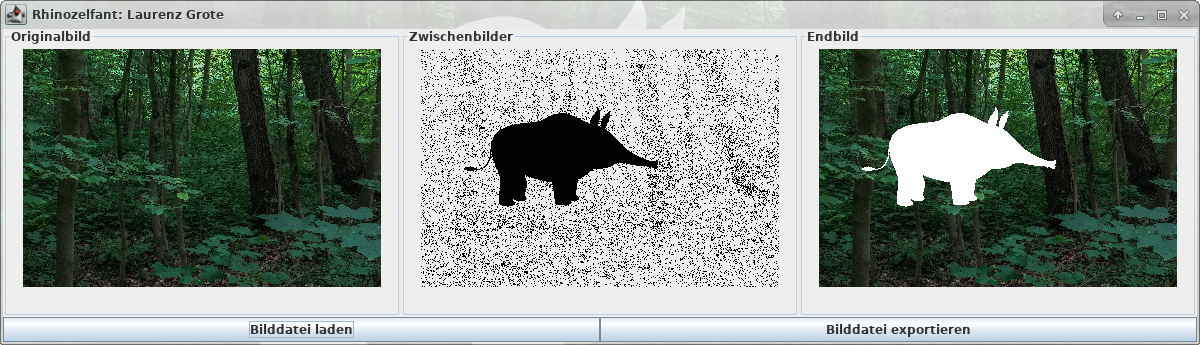
\includegraphics[width=0.8\textwidth]{bsp9}
% 	\caption {Beispielbild 9}
% \end{figure}

% Dieses Bild, welches neben dem eigentlichem Rhinozelfanten kaum größere Gruppen aus gleichfarbigen Feldern ausweist, ist ein Beispiel dafür, dass durch die geschachtelten Filter viel Laufzeit eingespart wird: Da fast alle Stellen wegen zu kurzer Länge früh verworfen werden, benötigt die Analyse nur ca. eine Sekunde.